\chapter{PACORA Framework}

\section{\pacora Architecture}\label{sys_design}

%II.	System Architecture
%		i.	Application Specific
%		ii.	Resources Matter
%		iii.	Measurement
%		iv.	Optimization
%	a.	Convex by construction
%		i.	Fairly representative of the actual system
%			1.	(Systems should be more convex)
%		ii.	Low Overhead
%	b.	Explanation of resources
%	c.	Performance Models Built Online
%		i.	Explanation of performance
%		ii.	When does it run?
%	d.	Penalty functions
%	e.	Dynamic Optimization
%		i.	When does it run?


%\pacora, which stands for Performance-Aware Convex Optimization for Resource Allocation, is a framework designed to determine the proper amount of each resource type to assign to each application.  For our purposes an application is the entity to which the operating system allocates resources: it can viewed as a complete application (\emph{e.g.,} a video player) or a component of an application (\emph{e.g.,} a music synthesizer) or a process (\emph{e.g.,} indexing).

\pacora is a framework designed to determine the proper amount of each
resource type to give each application.  For example, consider a video
conference scenario where each participant requires a separate,
performance-guaranteed video stream.  New participants may join the
conference and others may leave, increasing or decreasing the number
of streams running at any given time.  Simultaneously, participants
may be collaborating through web browsers, or watching shared video
clips and web searching, while their systems run compute-intensive
background tasks such as updates, virus scans, or file indexing.
Although it may be relatively straightforward to provide
responsiveness guarantees for individual applications such as video
streams, the real challenge is to do so without reserving excessive
resources, which will compromise system utilization or power
consumption. The purpose of \pacora is to dynamically assign resources
across multiple applications to guarantee responsiveness without
over-provisioning and to adapt allocations as the application mix
changes.

For our purposes an application is an entity to which the system
allocates resources: these can be a complete application (\emph{e.g.,}
a video player), a component of an application (\emph{e.g.,} a music
synthesizer), a background OS process (\emph{e.g.,} indexing), a job
in warehouse-scale computing, or a distributed application in a
distributed embedded system.

\pacora is designed for systems where resource allocation is separated
from scheduling.  This split enables the use of application-specific
scheduling policies, which have the potential to be easier to design
and more efficient than general-purpose schedulers that have to work
for everything.  This approach leaves the system to focus on the
problem of \emph{how much} of each resource type to assign to each
application.  In client machines, \pacora is used to make coarse-grain
resource-allocation decisions (\emph{e.g.,} cores and memory pages) at
the OS level, while the micro-management of these resources to run
application tasks is left to user-level runtimes such as Intel
Threaded Building Blocks~\cite{CoMa08} or Lithe~\cite{lithe}, and to
user-level memory managers.
%As a result, \pacora could be used to consolidate realtime systems.  Resources can be allocated to various realtime user-level schedulers such as Earliest-Deadline-First or Rate-Monotonic schedulers, eliminating the need in the case of many applications for a realtime OS designed around one of these schedulers.
In the cloud environment, \pacora allocates
resources (\emph{e.g.,} nodes and storage) to jobs, and scheduling is
left to other entities such as the MapReduce framework\cite{mapreduce}
or the node OS.  \pacora can also be used in a hypervisor to allocate
resources among guest OSes.

\pacora formulates resource allocation as an optimization problem
built from two types of application-specific functions: a
response-time function and a penalty function. The response-time
function represents the performance of the application with different
resources, and is built with runtime measurements.  The penalty
function represents the user-level goals for the application
(\emph{i.e.,} the deadline and how important it is to meet). \pacora uses convex optimization\cite{BoVa} to
determine the ideal resource allocation across all active
applications.  The following subsections briefly introduce the primary
components of \pacora and the optimization formulation.

\subsection{Resources}

In our client system, resources are anything that the system can
``partition'' in hardware or software: specifically we use cores,
network bandwidth, cache ways, and memory pages in our system.
However, other resources could be easily added assuming they have QoS
enforcement mechanisms.  The other scenarios would have resources that
perform similar functions (compute, network, capacity), but at a
different scale. For warehouse-scale computing, resources are more
likely to be different types of nodes, network bandwidth, and
storage. For distributed embedded systems, resources would include
compute devices, link bandwidths, and memories.

\subsection{Response-Time Functions}

Response-time functions (RTF) represent the expected \emph{response
  time} of an application as a function of the resources allocated to
the application. The response time is an application-specific measure
of the performance of the application.  For example, the response time
of an application might be:
    \begin{itemize}\itemsep0pt \parskip0pt \parsep5pt
    \item The time from a mouse click to its result;
    \item The time to produce a frame;
    \item The time from a service request to its response;
    \item The time from job launch to job completion;
    \item The time to execute a specified amount of work.
    \end{itemize}

The RTFs are built to be convex functions.  All applications have a
function of the same form but the application-specific weights are set
using the performance history of the application.  RTFs are designed
to capture information such as how well an application scales with a
particular resource. As a result, RTFs naturally support
heterogeneity.  Each CPU or GPU type is simply viewed as a different
resource type by the system, and thus the RTFs will represent how
effectively an application uses a particular type of
core. Figure~\ref{sample_rtf} shows two example RTFs we have created
from applications we studied.

\begin{figure}[hb]
\includegraphics*[bb=0 0 360 360,width=.49\columnwidth]{Figures/bfs-fig.pdf}
\includegraphics*[bb=0 0 360
  360,width=.49\columnwidth]{Figures/streamcluster-fig.pdf}
\caption{\label{sample_rtf} Response Time Functions for a
  breadth-first search algorithm and streamcluster from PARSEC. We show two resource dimensions: cores and cache slices.}
\end{figure}

Equation~\ref{rtf_eq} below shows the RTF we use in \pacora.

\begin{equation}\label{rtf_eq}
\tau(w,a) = \tau_0 + \sum_{i\in n,j\in n}{\frac{w_{i,j}}{\sqrt{a_i * a_j}}}
\end{equation}

Here $\tau$ is the response time, $i$ and $j$ are
resource types, $n$ is the total number of resource types,
$a_{i}$ and $a_{j}$ are the allocations of resource types $i$
and $j$, and $w_{i,j}$ is the application-specific weight for
the term representing resources $i$ and $j$.
We choose this specific function because it is convex in the resources and in initial application studies
we found it models response time behavior accurately enough to allow the optimization to make good decisions.
In our experience the cross term weights (those with $i\neq j$) are almost always negligible and can be omitted.
The dimensionality of the function increases roughly linearly with the number of resource types.
The RTFs will be described further in Section~\ref{RTFs}.
Alternative models and the initial model evaluations are described in
\cite{pacora_tr}.
%Appendix~\ref{rtf_choice}.


\pacora assumes some amount of performance isolation between
applications.  In order for the RTFs to accurately reflect the
expected response times of the applications, it is important that the
response time does not change much as a function of the other
applications currently running on the machine.  However, the
performance isolation need not be completely perfect: all of our
evaluation was run on current x86 hardware with some shared resources,
and \pacora is still effective. Section~\ref{discuss} discusses
handling shared resources in more detail.

\subsection{Penalty Functions}
Penalty functions are designed to represent the user-level goals of
the application. They are similar to priorities but are functions of
the response time rather than simply values, so they can explicitly
represent deadlines.  Knowing the deadlines lets the system make
optimizations that are difficult in today's systems, such as running
just fast enough to make the deadline. Like priorities, the penalty
functions are set by the system on behalf of the user.

\pacora's penalty functions $\pi$ are non-decreasing piecewise-linear
functions of the response time $\tau$ of the form $\pi(\tau) = \max(0, (\tau - d)s)$
where $d$ represents the deadline of the application and $s$ (slope)
defines the rate the penalty increases as response time increases. For
applications without response-time constraints the deadline can be set
to $0$. Two representative graphs of this type appear in
Figures~\ref{f:pen1} and~\ref{f:pen2}.

%In a client operating system, management of penalty function modifications
%should be highly automated by the system to avoid unduly burdening the user.
%As an application grows or diminishes in importance, its penalty function can be modified accordingly.
%Adjustment is also likely to occur in transitions between operating scenarios.
%For example, when unplugging a device all of the background activities could have their slopes significantly reduced to save battery life.

\begin{figure}[hb]
\parbox{1.6in}{
\includegraphics*{Figures/Penalty1.eps}
\caption{\label{f:pen1}A penalty function with a response time constraint.}
}
\hspace{\fill}
\parbox{1.6in}{
\includegraphics*{Figures/Penalty2.eps}
\caption{\label{f:pen2}A penalty function with no response time constraint.}
}
\end{figure}

\subsection{Resource Allocation as Optimization}

\pacora formulates resource allocation as an optimization problem
designed to minimize the total penalty of the system. This approach is
analogous to minimizing user dissatisfaction with the user experience
due to missed deadlines in a client system, and minimizing the contract
penalties paid for violated SLAs in a cloud
system.

The optimization selects the allocations for all resources and
resource types at once.  This approach enables the system to make
tradeoffs between resource types.  For example, the system could
choose to allocate more memory bandwidth in lieu of on-chip cache, or
one large core instead of several small cores.  Given that all of the
resources allocated to an application contribute to the response time,
it would difficult to provide predictable response times for
applications by considering the allocation of only one resource type at a
time.

A succinct mathematical characterization of this resource allocation scheme is the following:
\begin{eqnarray*}
& \makebox[1in][r]{Minimize}   & \sum_{p\in P} {\pi_p(\tau_p(a_{p,1}\ldots a_{p,n}))}  \\
& \makebox[1in][r]{Subject to} & \sum_{p\in P} a_{p,r} \leq A_r, r = 1,\ldots n        \\
& \makebox[1in][r]{and}        & a_{p,r} \geq 0
\end{eqnarray*}
Here $\pi_p$ is the penalty function for application $p$,
$\tau_p$ is its response time function,
$a_{p,r}$ is the allocation of resource $r$ to application $p$,
and $A_r$ is the total amount of resource $r$ available.  Optimization details are described in Section~\ref{dyn_opt}.

\subsection{Convex Optimization}

If the penalty functions, response time functions, and resource
constraints were arbitrary, little could be done to optimize the total
penalty beyond searching at random for the best allocation.  However,
by framing our resource allocation problem as a \emph{convex
  optimization problem}\cite{BoVa}, two benefits accrue: an optimal
solution will exist without multiple local extrema, and fast,
incremental solutions will become feasible.

A constrained optimization problem is \emph{convex} if both the objective function to be minimized
and the constraint functions that define its feasible solutions are convex functions.
A function $f$ is convex if its domain is a convex set and
$f(\theta x + (1-\theta)y) \leq \theta f(x) + (1-\theta)f(y)$
for all $\theta$ between 0 and 1.
A set is convex if for any two points $x$ and $y$ in the set, the point
$\theta x + (1-\theta)y$
is also in the set for all $\theta$ between 0 and 1.
%If $f$ is differentiable, it is convex if its domain is an open convex set and
%$f(y) \geq f(x) + \nabla f^T\cdot(y-x)$ where $\nabla f$ is the gradient of $f$.
%Put another way, $f$ is convex if its first-order Taylor approximations
%are always global underestimates of its true value.

A convex optimization problem is one that can be expressed in this form:
\begin{eqnarray*}
& \makebox[1in][r]{Minimize}   & f_0(x_1,\ldots x_m)                              \\
& \makebox[1in][r]{Subject to} & f_i(x_1,\ldots f_m) \leq 0, i = 1,\ldots k        \\
& \makebox[1in][r]{where}      & \forall i \quad f_i:\Re^m \rightarrow \Re \mbox{ is convex.}
\end{eqnarray*}


\pacora's resource allocation problem can be transformed into a convex
optimization problem in the $m = |P|\cdot n$ variables $a_{p,r}$ as
long as the penalty functions $\pi_p$ are convex non-decreasing and
the response-time functions $\tau_p$ are convex.  We designed our
functions to meet these constraints, and proofs of their convexity can
be found in~\cite{pacora_tr}.
%Appendix~\ref{convex}. 
Note that the resource constraints
are affine and therefore convex; they can be rewritten as $\sum_{p\in
  P} (a_{p,r} - A_r) \leq 0$ and $-a_{p,r} \leq 0$.

The convex formulation makes the optimization scale linearly in the
number of resource types and the number of applications.  For client
operating systems with around 100 applications running and 10 resource
dimensions, the total number of variables in the optimization problem
is 1000---a very small problem which is solved in microseconds on
current systems.  Cloud systems could have many more than 100
applications running, but the problem size scales linearly and the
potential benefits of a good allocation should scale rapidly with the
size of the system.

\pacora also formulates RTF \emph{creation} as a convex optimization
problem, as explained in Section~\ref{RTFs}.

\subsection{Power and Energy}
In \pacora, we create an artificial application to represent the
interest in reducing system power and energy.  Application 0 is
designated the idle application and receives allocations of all
resources that are left idle, \emph{i.e.,} not allocated to other
applications.  The idle resources can be powered off or put to sleep
if possible to save power.

The ``response time'' for application 0, $\tau_0$, is artificially
defined to be the total system power consumption.
%This response function is affine and monotone nonincreasing in its arguments $a_{0,r}$.
The penalty function $\pi_0$ establishes a system tradeoff between
power and performance that will determine which resources are
allocated to applications to improve performance and which are left
idle.  The penalty function $\pi_0$ can be used to keep total system
power below the parameter $d_0$ to the extent the penalties of other
applications cannot overcome its penalty slope $s_0$. Both $s_0$ and
$d_0$ can be adjusted to reflect the current battery charge in mobile
devices. For example, as the battery depletes, $d_0$ could be decreased or $s_0$ increased
to force other applications to slow or cease execution.

%Additionally, application 0 functions as \emph{slack} variables in our optimization problem turning the resource bounds into equalities:
%\begin{equation}
%\sum_{p\in P} a_{p,r} - A_r = 0, r = 1,\dots n.
%\end{equation}

\section{Response Time Functions}\label{RTFs}
%III.	Application Functions
%	a.	Resource Value Functions
%		i.	Structure
%		ii.	Model Building Approach
%			1.	Who measures the data?
%	b.	Penalty Functions
%		i.	Where do the deadlines come from?
%		ii.	How do we set the slopes?
%	c.	Power Model


In this section, we describe the design of \pacora's RTFs in more detail.
RTFs describe an application's performance given its resource assignments.  These functions capture information about the performance impact of a particular resource to an application on the current hardware at a particular time. Without this information, it would be difficult for any resource allocation system to make informed decisions short of blindly trying a variety of allocations and picking the best one.

\subsubsection*{Modeling versus Interpolating} While it might have been possible to model response times by recording past values and interpolating among them, this idea has serious shortcomings:
\begin{itemize}
\item The multidimensional response time tables would be large;
\item Interpolation in many dimensions is computationally expensive;
\item The measurements will be noisy and require smoothing;
\item Convexity in the resources may be violated;
\item Gradient estimation will be slow and difficult.
\end{itemize}

Instead of interpolating, \pacora maintains a parameterized analytic response time model with the partial derivatives evaluated from the model \emph{a priori}. Application responsiveness is highly nonlinear for an increasing variety of applications like streaming media or gaming, thus requiring many data points to represent the response times without a model. Using models, each application can be described in a small number of parameters.  Models can be built from just a few data points and can naturally smooth out noisy data. Their gradients, needed by \pacora to solve the optimization problem efficiently, are easy to calculate.

\pacora models response times with functions that are convex by construction.
The specific function chosen for \pacora is shown in Equation~\ref{rtf_eq} above.
In this equation, the response time is modeled as a weighted sum of component terms,
roughly one per resource, where a term $w_i/a_i$ is the amount of work $w_i \geq 0$
divided by $a_i$, the allocation of the $i$th resource~\cite{Snav}.
For example, one term might model instructions executed divided by total processor MIPS;
another might model network accesses divided by bandwidth, and so forth.
%Asynchrony and latency tolerance may make response time components overlap partly or fully; and thus we added additional terms to represent the interactions between resources.

Such models are automatically convex in the allocations because $1/a$ is convex for positive $a$ and because a positively-weighted sum of convex functions is convex.  The models are also linear in the weights.

%It is obviously important to guarantee the positivity of the resource allocations. This guarantee can be enforced as the %allocations are selected during penalty optimization, or the response time model can be made to return $\infty$ if any allocation %is less than or equal to zero. This latter idea preserves the convexity of the model and extends its domain to all of $\Re^n$ and %consequently we used this approach in our implementation.
%The gradient $\nabla\tau$ is needed by the penalty optimization algorithm.
%Since $\tau$ is analytic, generic, and symbolically differentiable
%it is a simple matter to compute the gradient of $\tau$ once the model is defined.

\subsubsection*{Non-Convexity}
Forcing RTFs to be convex assumes that the actual response times are
close to convex. We find this to be a plausible requirement as
applications usually follow the ``Law of Diminishing Returns'' for
resource allocations.

However, there are examples of response time versus resource behavior that violate convexity.   For example, we have seen non-convex performance in applications when dealing with hyperthreads or memory pages.  For two of our applications, 5 hyperthreads resulted in significantly worse performance than either 4 or 6.  When studying some other applications, we found that particular numbers of memory pages, (\emph{e.g.,} 2K), resulted in much better performance than the adjacent page allocations.  Outliers and additional challenges to response time modeling are discussed in Section~\ref{discuss}.
%Avoiding (or seeking out) these allocations would add significant cost to the optimization problem.

Another kind of convexity violation can occur in memory allocation, where ``plateaus'' can sometimes occur as in Figure~\ref{f:plat}. Such plateaus are typically caused by adaptations within the application (\emph{e.g.,} adjusting the algorithm or output quality).
%to accommodate variable resource availability.  
The response time is really the \emph{minimum} of several convex functions depending on allocation, and the point-wise minimum that the application implements fails to preserve convexity.  The effect of the plateaus will be a non-convex penalty as shown in Figure~\ref{f:plateffect} and multiple extrema in the optimization problem will be a likely result. 



\begin{figure}[hb]
\parbox{1.6in}{
\includegraphics*{Figures/Plateau1.eps}
\caption{\label{f:plat}Response time function with some resource ``plateaus''.}
}
\hspace{\fill}
\parbox{1.6in}{
\includegraphics*{Figures/Plateau2.eps}
\caption{\label{f:plateffect}Net effect of the resource plateaus on the application penalty.}
}
\end{figure}
There are several ways to avoid this problem.  One is based on the observation that such response time functions will at least be \emph{quasiconvex}.  Another idea is to use additional constraints to explore convex sub-domains of $\tau$. Either approach adds significant computational cost, and we found that our simple convex models still resulted in high-quality resource allocations. Thus we chose not to implement any of these approaches.  Alternative approaches to handling non-convex behavior are described in~\cite{pacora_tr}. 

%\subsubsection*{Dynamically Changing Applications}
%
%
%\fix{changing apps}
%\fix{dynamic compilation}
%\fix{phases}
%Response time will commonly vary with time as a application changes phase and makes better or worse use of its resources.
%\fix{non-determinism}
%
%\fix{Input Variability}


\subsubsection*{Data Collection and Model Creation Time}
There are many ways to collect the response time data for
applications. The user-level runtime scheduler is one possible source,
or the operating system could measure progress using performance
counters.  In our implementation, applications report their own
measured values; however, this solution was chosen simply as a way to
test the validity of the concept.  In a production operating system it
may not be a good idea because applications could lie about their
performance.  In a single-operator datacenter environment this might be less of a concern.

There are also many different possible moments to create response time functions.  RTFs could be created in advance and distributed with the application. This approach could make lots of sense for app stores since most of them cater to just a few platforms. RTFs could also be crowd-sourced and built in the cloud, which has the advantage making it easy to collect a diverse set of training points.  However, all of these approaches lack adaptability.  As a result, we have chosen to implement two solutions that collect data directly from the user's machine.  The first approach is to adapt to the system by collecting all of the training points at application install time and building the model then.  The most highly adaptive approach collects data continuously as the application runs, uses the data to modify the model training set, and rebuilds the model.  A hybrid approach may be the most effective: applications can begin with a generic model and improve it over time. The remainder of this Section describes our model creation process in detail.
\subsection{Response Time Model Creation}
To create RTF models either at install time or online we use a convex
least-squares approach described below.  At install time, we use a
genetic algorithm, Audze-Eglasis Design of
Experiments\cite{bates-aes03}, to select the resource vectors to use
for training.  These vectors and their response times are fed into the
convex least-squares algorithm. Online model building uses data
from the application's response time history.

\subsubsection*{Least-Squares Minimization}
After enough measurements, discovery of the model parameters $w$ that define the function $\tau$
can be based on a solution to the over-determined linear system $t=Dw$,
where $t$ is a column vector of actual response times measured for the application
and $D$ is a matrix whose $i$th row $D_{i,*}$ contains the corresponding resource vector.
Estimating $w$ is relatively straightforward: a least-squares solution accomplished via
\emph{QR factorization}\cite{GoVL} of $D$ will determine the $w$ that minimizes the \emph residual error of
$\|Dw - t\|^2_2 =  \|Rw - Q^Tt\|^2_2$.
%The solution proceeds as follows:
%\begin{eqnarray*}
%t     &=& Dw  - \varepsilon    \\
%      &=& QRw - \varepsilon    \\
%Q^Tt  &=& Rw  - Q^T\varepsilon
%\end{eqnarray*}
%
The individual elementary orthogonal transformations, \emph{e.g.,} Givens rotations,
that triangularize $R$ by progressively zeroing out $D$'s sub-diagonal elements are simultaneously applied to $t$.
%The elements of the resulting vector $Q^Tt$ that correspond to zero rows in $R$ comprise $-Q^T\varepsilon$.
%Since $Rw$ exactly equals the upper part of $Q^Tt$, the upper part of $Q^T\varepsilon$ is zero. The residual error for the %$t_i$
%can be found by premultiplying $Q^T\varepsilon$ by $Q$.

%This formulation assumes a model norm $p = 1$. If a different model norm $p$ is desired, such as $p = 2$, we could first square %each measurement in $t$
%and each reciprocal bandwidth term in $D$ and then follow the foregoing procedure.
%The elements of the result $w$ will be squares as well, and the 2-norm of the difference in the squared quantities will be %minimized.  This is not the same as minimizing the 4-norm; what is being minimized is $1/2\|\mbox{diag}(Dww^TD^T - tt^T)\|^2_2$.

\subsection{On-line Response Time Modeling}
As resource allocation continues, more measurements will become available to augment $t$ and $D$.
Moreover, older data may poorly represent the current behavior of the application.
\pacora uses an incremental approach described below to replace old data and efficiently update RTFs.

\subsubsection*{Incremental Least-Squares}
What is needed is a factorization $\tilde{Q}\tilde{R}$ of a new matrix $\tilde{D}$
derived from $D$ by dropping a row, perhaps from the bottom,
and adding a row, perhaps at the top.
Corresponding elements of $t$ are dropped and added to form $\tilde{t}$.

The matrices $\tilde{Q}$ and $\tilde{R}$ can be generated by applying Givens rotations
as described in Section 12 of \cite{GoVL} to \emph{downdate} or \emph{update} the factorization
much more cheaply than recomputing it \emph{ab initio}.
The method requires retention and maintenance of $Q^T$ but not of $D$.
Every update in \pacora is preceded by a downdate that makes room for it.
Downdated rows are \emph{not} always the oldest (bottom) ones, but
an update always adds a new top row.
For several reasons, the number of rows $m$ in $R$
will be at least twice the number of columns $n$.
Rows selected for downdating will always be in the lower $m - n$ rows of $R$,
guaranteeing that the most recent $n$ updates are always part of the model.

%\subsubsection*{Non-Negativity}
%\begin{figure*}[!t]
%	\begin{center}	
%%		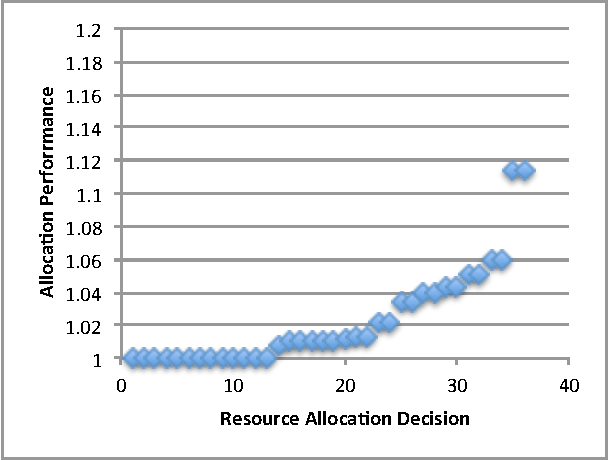
\includegraphics[width=.45\textwidth]{cluster_decision_points.pdf}
%		\caption{Performance of \pacora's NNLS algorithm}
%		\label{model_build_perf}
%	\end{center}
%\end{figure*}

To guarantee convexity of the RTF, the solution $w$ to $t \approx QRw$ must have no negative components.
Intuitively, when a resource is associated with more than a single $w_j$
or when the measured response time increases with allocation then negative $w_j$ may occur. \emph{Non-negative Least-Squares} problems (NNLS) are common linear algebra, and there are several well-known techniques\cite{ChPl}.
However since \pacora's online model maintenance calls for
incremental downdates and updates to rows of $Q^T$, $Q^Tt$ and $R$,
the NNLS problem is handled with a scheme
based on the \emph{active-set} method\cite{LaHa} that
also downdates and updates the \emph{columns} of $R$ incrementally,
roughly in the spirit of Algorithm~3 in~\cite{LuDu}.
However, \pacora's algorithm cannot ignore downdated columns of $R$
because subsequent \emph{row} updates and downdates must have due effect
on these columns to allow their later reintroduction via column updates as necessary.
This problem is solved by leaving the downdated columns in place,
skipping over them in maintaining and using the QR factorization.

The memory used in maintaining a model with $n$ weights is modest, $24n^2 + 21n + \textrm{O}(1)$ bytes.
For $n = 8$ this is under 2 KB, fitting nicely in L1 cache.
Our NNLS implementation takes \SI{4}{\micro\second} per update-downdate pair in \tess.
%Figure~\ref{model_build_perf} shows the performance of \pacora's NNLS algorithm.

\subsubsection*{Model Rank Preservation}
If care is not taken in downdating $R$, its rows may become so linearly dependent,
perhaps from repetitive resource allocations,
that determining a unique $w$ is impossible.
The rank of $R$ depends on both the resource optimization trajectory and the
choices made in the row downdate-update algorithm.
\pacora exploits the latter idea and simply avoids downdating any row that will make $R$ rank-deficient.

\subsubsection*{Outliers and Phase Changes}

%\begin{figure*}[!t]
%	\begin{center}	
%%		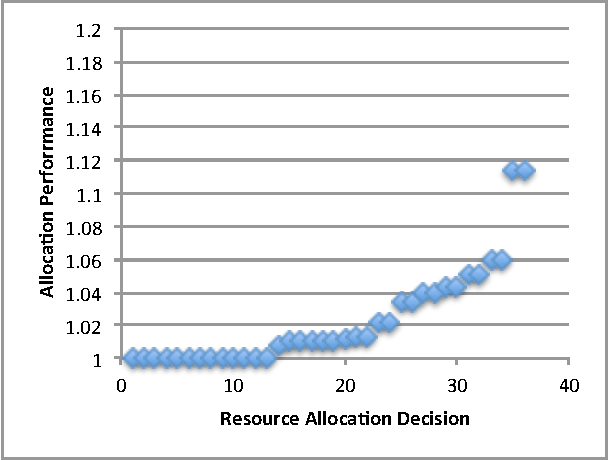
\includegraphics[width=.45\textwidth]{cluster_decision_points.pdf}
%		\caption{\pacora's online model creation algorithm adapting to a video application changing phases}
%		\label{phase_change}
%	\end{center}
%\end{figure*}

Some response time measurements may be ``noisy'' or even erroneous.
A weakness of least-squares modeling is the high importance it gives to outlying values.
On the other hand, when an application changes phase it is important to adapt quickly,
and what looks like an outlier when it first appears may be a harbinger of change.
What is needed is a way to discard either old or outlying data
with a judicious balance between age and anomaly.

The downdating algorithm accomplishes this by weighting the errors in $\varepsilon = Q(Q^Tt - Rw)$
between the predicted response times $\tau$ and the measured ones $t$ by a factor
that increases exponentially with the age $g(i)$ of the error $\varepsilon_i$.
Age can be modeled coarsely by the number of time quanta of some size since the measurement;
\pacora simply lets $g(i) = i$.
The weighting factor for the $i$th row is then $\eta^{g(i)}$ where $\eta$ is a constant somewhat greater than 1.
The candidate row to downdate is the row with the largest weighted error, \emph{i.e.,}
$dd = \arg\max_i |\varepsilon_i| \cdot \eta^{g(i)}$ and that does not reduce the rank of $R$.
%Figure~\ref{phase_change} shows \pacora's model creation algorithm adapting to a video application changing phases.


\subsubsection*{Power Response Modeling}
Recall that we manage power and battery energy with an artificial application named application 0 which receives all resources not allocated to other applications. Application 0's "response time" function is similar to the other applications' RTFs.  The function inputs are resource allocations just as with the other applications.  However, the function output is system power rather than response time.   To create the RTF, system power can be measured directly from on-chip energy counters in systems where they are available or from a power meter.  These models can be built in advance, during a training phase or online while the system runs, just as with the application RTFs.  Alternatively, the model could be part of the operating system's platform-specific information.

Although system power may not be perfectly convex in reality, forcing it to be convex is reasonable because idling a resource should not increase power.  As a result, application 0 still fufills its purpose of keeping applications from using additional resources that have poor performance/power ratios.

\section{Response Time Model Design}\label{rtf_choice}

\subsection*{Alternative Resource Representations}
Asynchrony and latency tolerance may make response time components overlap partly or fully;
if the latter, then the maximum of the terms might be more appropriate than their sum.
The result will still be convex, though, as will any other norm including the 2-norm,
\emph{i.e.} the square root of the sum of the squares.
This last variation could be viewed as a ``partially overlapped'' compromise between
the 1-norm (sum) describing no overlap and the $\infty$-norm (maximum) describing full overlap.

Sometimes a response time component might be better modeled by a term involving a combination of resources.
For example, response time due to memory accesses might be approximated
by a combination of memory bandwidth allocation $b_{r1}$ and cache allocation $m_{r2}$.
Such a model could use the geometric mean of the two allocations in the denominator,
\emph{viz.} $w_{r1,r2}/\sqrt{b_{r1}\cdot m_{r2}}$, without compromising convexity.

This scheme also accommodates non-bandwidth resources such as memory,
the general idea being to roughly approximate ``diminishing returns'' in the response time with increasing resources.
For clarity's sake, rather than using $a_r$ indiscriminately for all allocations,
we will denote an allocation of a bandwidth resource by $b_r$ and of a memory resource by $m_r$.
This begs the question of how memory affects the response time.
The effect is largely indirect.
Memory permits exploitation of temporal locality and thereby \emph{amplifies} associated bandwidths.
For example, additional main memory may reduce the need for storage or network bandwidth,
and of course increased cache capacity may reduce the need for memory bandwidth.
The effectiveness of cache in reducing bandwidth was studied by
H. T. Kung\cite{Kung}, who developed tight asymptotic bounds on the bandwidth amplification
factor $\alpha(m)$ resulting from a quantity of memory $m$ acting as cache for a variety of computations.
He shows that
\begin{displaymath}
\begin{array}{lll}
\alpha(m) &= \Theta(\sqrt m) & \mbox{for dense linear algebra solvers} \\
          &= \Theta(m^{1/d}) & \mbox{for d-dimensional PDE solvers} \\
          &= \Theta(\log m)  & \mbox{for comparison sorting and FFTs} \\
          &= \Theta(1)       & \mbox{when temporal locality is absent}
\end{array}
\end{displaymath}

For these expressions to make sense, the argument of $\alpha$ should be dimensionless and greater than 1.
Ensuring this might be as simple as letting it be the number of memory resource quanta
(\emph{e.g.} hundreds of memory pages) assigned to the application.
If a application shows diminishing bandwidth amplification as its memory allocation increases, this can be accommodated:
\begin{displaymath}
\alpha(m) = \min(c_1\alpha_1(m),c_2\alpha_2(m)),\;c_1,c_2 \geq 0
\end{displaymath}

Each bandwidth amplification factor might be described by one of the functions above
and included in the denominator of the appropriate component in the response time function model.
For example, the storage response time component for the model of an out-of-core sort application might be
the quantity of storage accesses divided by the product of the storage bandwidth allocation and $\log m$,
the amplification function associated with sorting given a memory allocation of $m$.
Amplification functions for each application might be learned from response time measurements
by observing the effect of varying the associated memory resource while keeping the bandwidth allocation constant.
Alternatively, redundant components, similar except for amplification function, could be included in the model
to let the model fitting process decide among them.

\subsection*{Stochastic Models}

\subsection*{Initial Model Evaluation}


\section{Problem Convexity}\label{convex}

\subsection*{Penalty Function Convexity}
A few facts about convex functions will be useful in what follows.
First, a \emph{concave} function is one whose negative is convex.
Maximization of a concave function is equivalent to minimization of its convex negative.
An affine function, one whose graph is a straight line in two dimensions or a hyperplane in n dimensions,
is both convex and concave.  A non-negative weighted sum or point-wise maximum (minimum) of convex (concave) functions is convex (concave), as is either kind of function composed with an affine function.  The composition of a convex non-decreasing (concave non-increasing) scalar function with a convex function remains convex (concave).

Each penalty function $\pi$ is the pointwise maximum of two affine functions and is therefore convex.
Moreover, since each penalty function is scalar and nondecreasing,
its composition with a convex response time function will also be convex.

\subsection*{Response Time Convexity}
We now show that response time functions $\tau$ including the various bandwidth amplification functions are convex
in both the bandwidth and memory resources $b_r$ and $m_r$ given any of the possibilities we have considered.
Since norms preserve convexity, this reduces the question to proving each term in the norm is convex.
Since all quantities are positive and both maximum and scaling by a positive constant preserve convexity,
\begin{eqnarray*}
\lefteqn{w/(b\cdot\min(c_1\alpha_1(m),c_2\alpha_2(m)))}   \\
&=& \max(w/(b\cdot c_1\alpha_1(m)),w/(b\cdot c_2\alpha_2(m))).
\end{eqnarray*}
It therefore only remains to show that both $1/\sqrt{b\cdot m}$ and $1/(b\cdot\alpha(m))$ are convex in $b$ and $m$.

A function is defined to be \emph{log-convex} if its logarithm is convex.
A log-convex function is itself convex because exponentiation preserves convexity,
and the product of log-convex functions is convex because the log of the product is the sum of the logs,
each of which is convex by hypothesis.
Now $1/b$ is log-convex for $b > 0$ because $-\log b$ is convex on that domain.
In a similar way, $\log(1/\sqrt{b\cdot m}) = -(\log b + \log m)/2$
and $\log m^{-1/d} = -(\log m)/d$ are convex.
Finally, $\log (1/\log m)$ is convex because its second derivative is positive for $m > 1$:
\begin{eqnarray*}
\frac{d^2}{dm^2}\log (1/\log m) &=& \frac{d^2}{dm^2}(-\log\log m)  \\
                                  &=& \frac{d}{dm}\left(\frac{-1}{m\log m}\right) \\
                                  &=& \frac{1 + \log m}{(m\log m)^2}.
\end{eqnarray*}

Summing up, a response time function for a application might be modeled by the convex function
\begin{eqnarray*}
\tau(w,b,\alpha,m) &=& \sqrt[p]{\sum_j \left(\frac{w_j}{b_j\cdot\alpha_j(m_j)}\right)^p}  \\
                   &=& \|\mbox{diag} wd^T \|_p
\end{eqnarray*}
where the $w_j$ are the parameters of the model (the quantities of work) to be learned,
the components of $d$ satisfy $d_j = 1/(b_j\cdot\alpha_j(m_j))$,
the $b_j$  are the allocations of the bandwidth resources,
the $\alpha_j$ are the bandwidth amplification functions (also to be learned),
the $m_j$ are the allocations of the memory or cache resources that are responsible for the amplifications.
This formulation allows the application response time $\tau$ to be modeled as the $p$-norm of
the component-wise product of a vector $d$ that is computed from the resource allocation
and a learned vector of work quantities $w$.

\subsection*{Handling Quasiconvex Response Time Functions}

There are examples of response time versus resource behavior that violate convexity.  One such example sometimes occurs in memory allocation, where ``plateaus'' can sometimes be seen as in Figure~\ref{f:plat}.

Such plateaus are typically caused by algorithm adaptations within the application to accommodate variable resource availability.  The response time is really the \emph{minimum} of several convex functions depending on allocation and the point-wise minimum that the application implements fails to preserve convexity.  The effect of the plateaus will be a non-convex penalty as shown in Figure~\ref{f:plateffect} and multiple extrema in the optimization problem will be a likely result.

There are several ways to avoid this problem.  One is based on the observation that such response time functions
will at least be \emph{quasiconvex}.  A function $f$ is quasiconvex if all of its \emph{sublevel sets}
$S_\ell = \{x | f(x) \leq \ell\}$ are convex sets.
Alternatively, $f$ is quasiconvex if its domain is convex and
\begin{displaymath}
f(\theta x + (1-\theta)y) \leq \max(f(x),f(y)), 0 \leq \theta \leq 1
\end{displaymath}

Quasiconvex optimization can be performed by selecting a threshold $\ell$ and replacing the objective function
with a convex constraint function whose sublevel set $S_\ell$ is the same as that of $f$.
Next, one determines whether there is a feasible solution for that particular threshold $\ell$.
Repeated application with a binary search on $\ell$ will reduce the level of feasibility
until the solution is approximated well enough.

Another idea is to use additional constraints to explore convex sub-domains of $\tau$.
For example,the affine constraint $a_{p,r} - \mu \leq 0$ excludes application $p$ from any assignment of resource $r$ exceeding $\mu$.  Similarly, $\mu - a_{p,r} \leq 0$ excludes the opposite possibility.
A binary (or even linear)search of such sub-domains could be used to find the optimal value.




